\documentclass[../../main.tex]{subfiles}
\begin{document}
\section{Cantilever plate model}\label{sec:FEM:Plate}
Consider a rectangular cantilever Reissner-Mindlin plate model with a rectangular cross-section.

\subsubsection{Reference configuration for a rectangular plate}
Let $\left\{e_1,e_2\right\}$ be a right-handed orthonormal basis for $R^2$. Although this basis seems identical to the two-dimensional beam in section \ref{sssec:2D_Model:RefConf}, it is fact different. It would be more appropriate to use $e_1$ and $e_3$ for this plate model. However the use of $e_1$ and $e_2$ is kept to reiterate that this is in fact a two-dimensional model.

Denote the elastic body as $\Omega \in R^2$ with the reference point $(0,0)$. For a rectangular plate,
\begin{eqnarray*}
	\Omega = \left \{ x \in R^2 \ | \ 0 \leq x_1 \leq 1, \ 0 \leq x_2 \leq b \right \}.
\end{eqnarray*}
Let $\partial \Omega$ denote the boundary of plate. The boundary $\partial \Omega$ can be divided into four distinct lines.

\noindent\begin{minipage}{.5\linewidth}
	\begin{eqnarray*}
		\Sigma:& \quad x_1 &= 0\\
		\Gamma_3:& \quad x_1 &= 1
	\end{eqnarray*}
\end{minipage}%
\begin{minipage}{.5\linewidth}
	\begin{eqnarray*}
		\Gamma_0:& \quad x_2 &= 0\\
		\Gamma_1:& \quad x_2 &= b
	\end{eqnarray*}
\end{minipage}

Similar to the two and three-dimensional cantilever models, this notation implies that the plate is clamped at $\Sigma$ and free hanging at $\Gamma$.

\subsubsection{Cantilever plate model}
Consider a rectangular Reissner-Mindlin plate clamped rigidly to a surface at $\Sigma$ and free hanging on the remaining edges. This plate model is presented in section \ref{ssec:P_Model:ModelProblems} as Problem P-1.

\begin{figure}[h!]
	\centering
	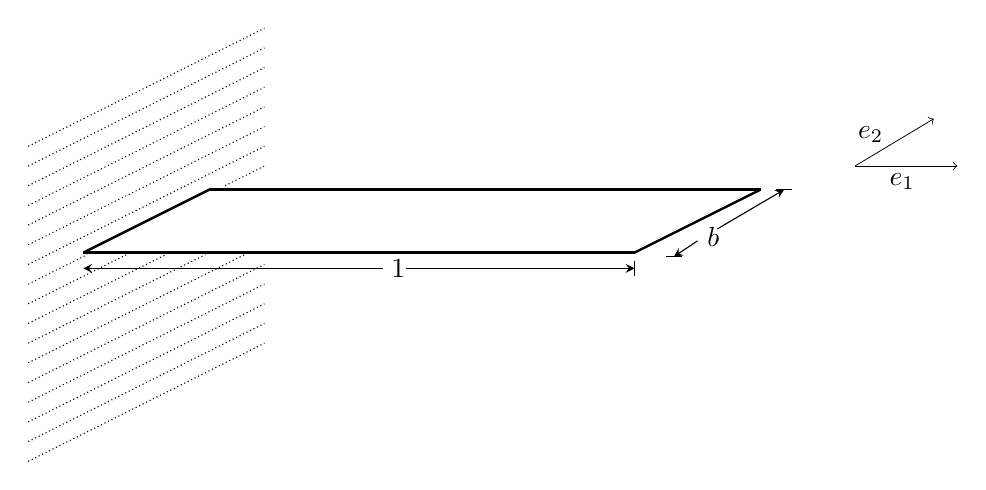
\begin{tikzpicture}

		\draw[line width = 0.3mm] (-0.8,-0.1) -- (6.2,-0.1);
		\draw[line width = 0.3mm] (0.8,0.7) -- (7.8,0.7);
		\draw[line width = 0.3mm] (-0.8,-0.1) -- (0.8,0.7);
		\draw[line width = 0.3mm] (6.2,-0.1) -- (7.8,0.7);



		\draw[scale=0.5, domain=-3:3, smooth, variable=\x,densely dotted] plot ({\x}, {0.5*\x+4});
		\draw[scale=0.5, domain=-3:3, smooth, variable=\x,densely dotted] plot ({\x}, {0.5*\x+3.5});
		\draw[scale=0.5, domain=-3:3, smooth, variable=\x,densely dotted] plot ({\x}, {0.5*\x+3});
		\draw[scale=0.5, domain=-3:3, smooth, variable=\x,densely dotted] plot ({\x}, {0.5*\x+2.5});
		\draw[scale=0.5, domain=-3:3, smooth, variable=\x,densely dotted] plot ({\x}, {0.5*\x+2});
		\draw[scale=0.5, domain=-3:3, smooth, variable=\x,densely dotted] plot ({\x}, {0.5*\x+1.5});
		\draw[scale=0.5, domain=-3:3, smooth, variable=\x,densely dotted] plot ({\x}, {0.5*\x+1});

		\draw[scale=0.5, domain=-3:-1.5, smooth, variable=\x,densely dotted] plot ({\x}, {0.5*\x+0.5});
		\draw[scale=0.5, domain=2:3, smooth, variable=\x,densely dotted] plot ({\x}, {0.5*\x+0.5});

		\draw[scale=0.5, domain=-3:-0.5, smooth, variable=\x,densely dotted] plot ({\x}, {0.5*\x});
		\draw[scale=0.5, domain=-3:0.5, smooth, variable=\x,densely dotted] plot ({\x}, {0.5*\x-0.5});
		\draw[scale=0.5, domain=-3:1.5, smooth, variable=\x,densely dotted] plot ({\x}, {0.5*\x-1});
		\draw[scale=0.5, domain=-3:2.5, smooth, variable=\x,densely dotted] plot ({\x}, {0.5*\x-1.5});
		\draw[scale=0.5, domain=-3:3, smooth, variable=\x,densely dotted] plot ({\x}, {0.5*\x-2});
		\draw[scale=0.5, domain=-3:3, smooth, variable=\x,densely dotted] plot ({\x}, {0.5*\x-2.5});
		\draw[scale=0.5, domain=-3:3, smooth, variable=\x,densely dotted] plot ({\x}, {0.5*\x-3});
		\draw[scale=0.5, domain=-3:3, smooth, variable=\x,densely dotted] plot ({\x}, {0.5*\x-3.5});
		\draw[scale=0.5, domain=-3:3, smooth, variable=\x,densely dotted] plot ({\x}, {0.5*\x-4});

		\node at (7.2,0.1) {$b$};
		\draw[-stealth] (7.25,0.2) -- (8.1,0.7);
		\draw (8,0.7) -- (8.2,0.7);
		\draw[-stealth] (7,0.05) -- (6.7,-0.15);
		\draw (6.6,-0.15) -- (6.8,-0.15);

		\node at (3.2,-0.3) {$1$};
		\draw[stealth-] (-0.8,-0.3) -- (3,-0.3);
		\draw[stealth-] (6.2,-0.3) -- (3.3,-0.3);
		\draw (6.2,-0.2) -- (6.2,-0.4);

		%\node at (6.5,0.3) {$\Sigma_1$};
		%\node at (0.51,0.3) {$\Sigma_0$};
		%\node at (3.2,0.05) {$\Gamma_0$};
		%\node at (3.6,0.5) {$\Gamma_1$};
		%\node at (-0.7,-0.3) {$(0,0)$};

		\draw[line width = 0.1mm,->] (9,1) -- (10,1.6);
		\draw[line width = 0.1mm,->] (9,1) -- (10.3,1);
		\node at (9.2,1.4) {$e_2$};
		\node at (9.6,0.8) {$e_1$};


		\draw[line width = 0.2mm] (0.8,0.7) -- (7.8,0.7);
		\draw[line width = 0.2mm] (-0.8,-0.1) -- (0.8,0.7);
		\draw[line width = 0.2mm] (6.2,-0.1) -- (7.8,0.7);

	\end{tikzpicture}
	\caption{Two-dimensional cantilever Reissner-Mindlin plate}
\end{figure}
\FloatBarrier

In section \ref{ssec:P_Model:ModelProblems} the variational problem for the cantilever Reissner-Mindlin plate is defined by Problem P-1V. For convenience, the relevant results from section \ref{ssec:P_Model:ModelProblems} are repeated.

\subsubsection{Problem P-1V}
Find a function $u = \langle w, \psi \rangle$, such that for all $t>0$, $u \in T_1({\bar{\Omega}}) \times T_2({\bar{\Omega}})$ and the following equations are satisfied
\begin{eqnarray}
	c(u,\phi) &=& -b(u,\phi) + (Q,\phi), \label{eq:P_Model:ProblemP1V1}
\end{eqnarray} with $\phi = \langle v, \phi \rangle  \in T_1({\bar{\Omega}}) \times T_2({\bar{\Omega}})$ an arbitrary function.\\

With the test function spaces
\begin{eqnarray*}
	T_1(\bar{\Omega}) & = & \left \{v \in C^1(\bar{\Omega})\ | \ v = 0 \textrm{ on } \Sigma_0\right\},\\
	T_2(\bar{\Omega}) & = & \left \{ \phi = \left[ \phi_1 \ \phi_2 \right]^T \ | \ \phi_1, \phi_2 \in C^1(\bar{\Omega}), \ \phi_1 = \phi_2 = 0 \textrm{ on } \Sigma_0 \right\}.
\end{eqnarray*}

The bilinear forms and integral function defined by

\begin{eqnarray*}
	b(u,\phi) & = & \int_\Omega \boldsymbol{Q} \cdot \nabla v \ dA + \int_{\Omega} \textrm{Tr}(M\Phi) \ dA,\\
	c(u,\phi) & = & \int_\Omega h (\partial_t^2 w) v \ dA + \int_\Omega I (\partial_t^2 \psi) \cdot \phi \ dA \\
	(f,g) &=& -\int_{\Omega} f\cdot g \ dA \label{eq:2D_Model:Bilinear_int}
\end{eqnarray*}

Using the definition of the reference configuration, the constitutive equations and the bilinear form $b$ can be rewritten as follows.

\subsubsection{Constitutive Equations}
\begin{eqnarray}
	\boldsymbol{Q} & = & h(\nabla w + \boldsymbol{\psi}) \label{eq:P_Model:CE1D}\\
	M_{11} & = & \frac{1}{2\beta(1-\nu^2)} \left[ 2(\partial_1\psi_1 + \nu \partial_2 \psi_2 \right] \label{eq:P_Model:CE2D}\\
	M_{12} = M_{21} & = & \frac{1}{2\beta(1-\nu^2)} \left[ (1-\nu)(\partial_1\psi_2 + \partial_2 \psi_1) \right] \label{eq:P_Model:CE3D}\\
	M_{11} & = & \frac{1}{2\beta(1-\nu^2)} \left[ 2(\partial_2 \psi_2 + \nu \partial_1 \psi_1)\right] \label{eq:P_Model:CE4D}
\end{eqnarray}

\subsubsection{Bilinear Form}
\begin{eqnarray*}
b(u,\phi) & = & \int_\Omega \boldsymbol{Q} \cdot \nabla v \ dA + \int_{\Omega} \textrm{Tr}(M\Phi) \ dA,\\
	& + & \frac{1}{\beta(1-\nu^2)}\int_{\Omega} (\partial_1\psi_1 + \nu\partial_2\psi_2)\partial_1\phi_1+ (\partial_2\psi_2 + \nu\partial_1\psi_1)\partial_2\phi_2 \ dA,\\
	& + & \frac{1}{2\beta(1+\nu)}\int_{\Omega} (\partial_1\psi_2+\partial_2\psi_1)(\partial_1\phi_2+\partial_2\psi_1) \ dA.\\
\end{eqnarray*}

\subsection{Weak variational form}
Similar to Section 2.1, the weak variational form for Problem P-1 can be derived from Problem P-1V.

\subsubsection{Bilinear forms}
From the bilinear form, we have
\begin{eqnarray*}
	b(f_2,g_2) & = & \frac{1}{\beta(1-\nu^2)}\iint_{\Omega} (\partial_1f_{2,1} + \nu\partial_2f_{2,2})\partial_1g_{2,1}+ (\partial_2f_{2,2} + \nu\partial_1f_{2,1})\partial_2g_{2,2} \ dA,\\
	& + & \frac{1}{2\beta(1+\nu)}\iint_{\Omega} (\partial_1f_{2,2}+\partial_2f_{2,1})(\partial_1g_{2,2}+\partial_2 g_{2,1}) \ dA
\end{eqnarray*}

For all $f,g \in T_1(\Omega)\times T_2(\Omega) $, define the bilinear forms
\begin{eqnarray*}
	c(f,g) & = & h(f_1,g_1)_{\Omega} + I(f_2,g_2)_{R^2} \\
	b^*(f,g) & = & b(f_2,g_2) + h(\nabla f_1 + f_2, \nabla g_1 + g_2)_{R^2}
\end{eqnarray*}
where the integrals are defined by
\begin{eqnarray*}
	(f_1,g_1)_{\Omega} & = & \iint_\Omega f_1 g_1 \ dA,\\
	(f,g)_{R^2} & = & \iint_\Omega f \cdot g \ dA.
\end{eqnarray*}

Define $V_1(0,1)$ as the closure of $T_1(0,1)$ in $H^1(0,1)$ and $V_2(0,1)$ as the closure of $T_2(0,1)$ in $H^1(0,1)^2$.\\

Denote the space $X = L^2(0,1)\times L^2(0,1)^2$ as a setting for Problem P-1V. A natural inner product for $X$ is $(f,g)_X = (f_1,g_1)_{\Omega} + (f_2,g_2)_{R^2}$.  Define $W$ as the space $X$ with the inner product $c$ and $V = V_1(0,1) \times V_2(0,1)$

\subsubsection{Problem Plate-1W}
Find a function $u$ such that for all $t>0$, $u(t) \in V$, $u'(t) \in V$ and $u''(t) \in W$, satisfying the following equation
\begin{eqnarray}
	c(u''(t),v) + b^*(u(t),v) & = & (f(t),v)_{\Omega} \ \ \ \textrm{ for each } v \in V,
\end{eqnarray} with $u(0)= u_0 = \langle w_0, \boldsymbol\psi_0 \rangle$, and $u'(0)= u_1 = \langle w_1, \boldsymbol\psi_1 \rangle$.

See Chapter 2 for the existence theory.

\subsection{Galerkin approximation}
To discretise the body $\Omega$, the same shapes as in section \ref{ssec:2D_Model:Galerkin} are used.

Divide the reference configuration $\Omega$ into a rectangular grid of elements, such that there are $n = n_1 \times n_2$ nodes.

Define a set of $n$-dimensional linear independent basis functions. The basis functions can be defined by the set $$B = \left\{\langle\phi_1, 0\rangle, \langle\phi_2, 0\rangle,...,\langle\phi_{n}, 0 \rangle,\langle 0,\phi_1\rangle,\langle 0 ,\phi_2\rangle,...,\langle 0,\phi_{n}\rangle \right\}.$$ 

These basis functions are piecewise Hermite bi-cubic basis functions.

Since there are two test function spaces, $T_1(\Omega)$ and $T_2(\Omega)$, two different sets of admissible basis functions are required. Denote the admissible basis functions for $T_1(\Omega)$ by $\delta^1_j$ where each $\delta^1_j$ is a unique element of B. The set of admissible basis functions that satisfies $T_1(\Omega)$ can be defined as $A_1 = \left\{\delta^1_1, \delta^1_2,..., \delta^1_{k_1} \right\}$ for a $k_1 \leq 2n$. Similarly for $T_2(\Omega)$, the set of admissible basis functions can be defined as $A_2 = \left\{\delta^2_1, \delta^2_2,..., \delta^2_{k_2} \right\}$ for a $k_2 \leq 2n$.

Define the two spaces
\begin{eqnarray*}
	S^h_1 & = & \textrm{span}\left(\left\{\delta^1_i \ | \ i = 1,2,...,k_1 \right\} \right),\\
	S^h_2 & = & \textrm{span}\left(\left\{\delta^2_i \ | \ i = 1,2,...,k_2 \right\} \right).
\end{eqnarray*}
For each function $u^h \in S_1^h$ and each function $\psi^h \in S_2^h$, $u^h$ can be expressed as
\begin{eqnarray*}
	w^h = \sum_{i = 1}^{k} w_i(t) \delta^*_{i}(x)
\end{eqnarray*} and $\psi^h$ can be expressed as
\begin{eqnarray*}
	\psi^h = \sum_{i = 1}^{k} \psi_i(t) \delta_{i}(x)
\end{eqnarray*}

Substitution of $u^h$ and $\psi^h$ into Problem P-1V, results in the following Galerkin approximation, denoted by Problem P-1G.

\subsubsection{Problem P-1G}
Find a function $u^h = \langle w^h, \psi^h \rangle$, such that for all $t>0$, $u^h \in S_1^h \times S_1^h$ and the following equations are satisfied
\begin{eqnarray}
	c(u^h,\phi_{i,j}) &=& -b(u^h,\phi_{i,j}) + (Q^I,\phi_{i,j}), \label{eq:P_Model:ProblemP1V1}
\end{eqnarray} with $\phi_{i,j} = \langle v_i, \phi_j \rangle$ for $i = 1,2,...,k_1$ and $j = 1,2,...,k_2$

\subsection{System of ordinary differential equations}\label{plate_fem_g}
The standard FEM matrices $K_{11}$, $K_{12}$, $K_{21}$, $K_{22}$ and $M_F$ where presented in section \ref{ssec:2DFEM:DE}. Even though the definition of $R^2$ is different in section \ref{sec:FEM:2D}, the definition of the matrices are the same and are not repeated here.

In addition to these matrices, the following standard FEM matrices are also required.

\subsubsection{FEM matrices}
\noindent\begin{minipage}{.5\linewidth}
	\begin{eqnarray*}
		{L_{1}}_{ij} & = & \iint_{\Omega} \phi_j \partial_1\phi_i
	\end{eqnarray*}
\end{minipage}%
\begin{minipage}{.5\linewidth}
	\begin{eqnarray*}
		{L_{2}}_{ij} & = & \iint_{\Omega} \phi_j \partial_2\phi_i
	\end{eqnarray*}
\end{minipage}

for $i,j = 1,2,...,p$.

Define the following matrices:

\noindent\begin{minipage}{.5\linewidth}
	\begin{eqnarray*}
		\mathbf{K11} & = & hK_{11}-hK_{22}\\
		\mathbf{K12} & = & hL_1\\
		\mathbf{K13} & = & hL_2\\
		\mathbf{K21} & = & hL_1^T\\
		\mathbf{K22} & = & AK_{11}+BK_{22}+h\mathbf{M}
	\end{eqnarray*}
\end{minipage}%
\begin{minipage}{0.8\linewidth}
	\begin{eqnarray*}
		\mathbf{K23} & = & A\nu K_{12}+BK_{21}\\
		\mathbf{K31} & = & hL_2^T\\
		\mathbf{K32} & = & A\nu K_{21}+BK_{12}\\
		\mathbf{K33} & = & AK_{22}+BK_{11}+h\mathbf{M}
	\end{eqnarray*}
\end{minipage}\\

with $A = \frac{1}{\beta(1-\nu^2)}$ and $B = \frac{1}{2\beta(1+\nu)}$.

Using the standard FEM matrices and the matrices $\mathbf{K11}$ to $\mathbf{K33}$, the following concatenated matrices are defined.


\begin{eqnarray}
	\begin{aligned}
		K & = &
		\begin{bmatrix}
			\mathbf{K11} & \mathbf{K12} & \mathbf{K13}\\
			\mathbf{K21} & \mathbf{K22} & \mathbf{K23}\\
			\mathbf{K31} & \mathbf{K32} & \mathbf{K33}
		\end{bmatrix}
	\end{aligned}
	\ \ \ \ \ \ \ \ \
	\begin{aligned}
		M & = &
		\begin{bmatrix}
			h\mathbf{M} & {O} & {O}\\
			{O} & I\mathbf{M} & {O}\\
			{O} & {O} & I\mathbf{M}
		\end{bmatrix}\label{3DB_23}
	\end{aligned}\label{eq:PFEM:K+M}
\end{eqnarray}


\begin{eqnarray}
	M_f & = &
	\begin{bmatrix}
		{M_F} & {O_F} & {O_F}\\
		{O_F} & {M_F} & {O_F}\\
		{O_F} & {O_F} & {M_F}
	\end{bmatrix}\label{eq:PFEM:M}
\end{eqnarray}
The matrices ${O}$ and ${O_F}$ are the zero matrices of the same size as $\mathbf{M}$ and $\mathbf{M_f}$ respectively.\\


Using \eqref{eq:PFEM:K+M} and \eqref{eq:PFEM:M}, Problem P-1G is rewritten as a system of ordinary differential equations. This system is referred to as Problem P-1ODE
\subsubsection{Problem P-1ODE}
Find function $\bar{u} \in S_1^h\times S_2^h$ such that
\begin{eqnarray}
	M\ddot{\bar{u}} & = & K\bar{u} + M_{f}Q^I \label{Plate_FEM_M}
\end{eqnarray}
With $\bar{u}$ in the form $\bar{u} = \langle w, \partial_1 w, \partial_2 w, \partial_{12} w, \psi_1, \partial_1 \psi_1, \partial_2 \psi_1, \partial_{12} \psi_1, \psi_2, \partial_1 \psi_2, \partial_2 \psi_2, \partial_{12} \psi_2 \rangle$.

\subsection{Eigenvalue problem}

The equation \eqref{Plate_FEM_M} is the same form as in section \ref{2dFEM_EP} for the two-dimensional elastic body. Therefore the derivation of the eigenvalue problem is identical. Denote the eigenvalue problem for Problem P-1 by Problem P-1E.
\subsubsection{Problem P-1E}
Find a vector function $\bar{u}$ and a number $\lambda$ such that
\begin{eqnarray}
	M\lambda{\bar{u}} & = & K\bar{u}.
\end{eqnarray}


\end{document}
\subsubsection{Accuracy of the eigenvalues}
Recall that there are $n = (n_1+1)(n_2+1)$ elements for a choice of positive integers $n_1$ and $n_2$. Table 5.1 and 5.2 show that increasing the number of elements, the accuracy of the eigenvalues increase.\\

Fix $h = 1/20$.


\begin{table}[htbp]
	\makebox[\textwidth]{
		\caption{Relative error of first 50 eigenvalues of Problem P-1. Bi-Cubic basis functions.}
		\begin{tabular}{|lc|cccccc|}
			\hline
			\multicolumn{8}{|c|}{Relative Error of Eigenvalues} \\
			\hline
			\multicolumn{2}{|c|}{$n_1$} & {20} & {25} & {30} & {35} & {40} & {45} \\
			\hline
			\hline
			{d = 0.25} & n     & {126} & {208} & {279} & {360} & {451} & {598} \\
			& Error & 7.993 $\times 10^{-3}$ & 2.699$\times 10^{-3}$ & 6.686$\times 10^{-4}$ & 2.713$\times 10^{-4}$ &
			1.246$\times 10^{-4}$ & 7.545$\times 10^{-5}$ \\
			\hline
			{d = 0.5} & n     & {231} & {364} & {496} & {684} & {861} & {1104} \\
			& Error & 2.656$\times 10^{-3}$ & 8.026$\times 10^{-4}$ & 2.379$\times 10^{-4}$ & 1.159$\times 10^{-4}$ & 4.225$\times 10^{-5}$ & - \\
			\hline
			{d =1} & n     & {441} & {676} & {961} & {1296} & {1681} & {2116} \\
			& Error & 1.255$\times 10^{-3}$ & 3.285$\times 10^{-4}$ & 1.228$\times 10^{-4}$ & 5.225$\times 10^{-6}$ & -     & - \\
			\hline
			{d = 1.25} & n     & {546} & {858} & {1209} & {1620} & {2091} & {2668} \\
			& Error & 8.608$\times 10^{-4}$ & 2.677$\times 10^{-4}$ & 9.040$\times 10^{-5}$ & -     & -     & - \\
			\hline
		\end{tabular}%
		\label{tab:addlabel}%
	}
\end{table}%

\FloatBarrier

In Table 5.1, the ratio between $n_1$ and $n_2$ are kept so that $\Delta x_1$ and $\Delta x_2$ are equal for all elements. So for any $n_1$, $n_2 = \lceil d n_1 \rceil$.\\

Table 5.1 shows that using bi-cubic basis functions, an accuracy of at least 4 significant digits can be obtained with minimal elements. It also shows that the number of elements have to be increased as the parameter $d$ is increased.




\subsubsection{Eigenvalues and eigenfunctions}
Fix $b =1$. Table 5.1 shows examples of the eigenvalues. The greater the ratio between $b$ and $h$ with $b>h$, the smaller the first eigenvalues become.
\begin{table}[!h]
	\centering
	\renewcommand{\arraystretch}{1.05}
	\begin{tabular}{|l||l|l|l|}
		\hline
		\multicolumn{4}{|l|}{Cantilever Plate Eigenvalues with $b = 1$.} \\ \hline
		i        & $h = 1/10$       & $h  = 1/20$      & $h = 1/30$      \\ \hline
		1        & 0.0336           & 0.00845          & 0.00381         \\
		2        & 0.186            & 0.0496           & 0.0224          \\
		3        & 1.15             & 0.313            & 0.142          \\
		4        & 1.86             & 0.506            & 0.230           \\
		5        & 2.28             & 0.643            & 0.294            \\
		6        & 6.45             & 1.92             & 0.887            \\
		7        & 8.37             & 2.50             & 1.15            \\
		8        & 9.29             & 2.74             & 1.26            \\
		9        & 10.8             & 3.29             & 1.53            \\
		10       & 17.4             & 5.49             & 2.58            \\ \hline
	\end{tabular}
	\caption{First 10 eigenvalues of a cantilever plate, with $b = 1$ and varying values for $h$.}
\end{table}

\subsubsection{Shapes of modes/eigenfunctions**}
Figure 5.1 show examples of several mode shapes of a cantilever plate model.
\begin{figure}[h!]
	\centering
	\begin{minipage}[b]{0.4\linewidth}
		\includegraphics[width=60mm]{BeamType.png}
		\subcaption{Beam Type}
		\label{fig:minipage1}
	\end{minipage}
	\quad
	\begin{minipage}[b]{0.4\linewidth}
		\includegraphics[width=60mm]{2DType.png}
		\subcaption{2-Dimensional Wave}
		\label{fig:minipage2}
	\end{minipage}
	\quad
	\begin{minipage}[b]{0.4\linewidth}
		\includegraphics[width=60mm]{TwistType.png}
		\subcaption{Twisting}
		\label{fig:minipage2}
	\end{minipage}
	\quad
	\begin{minipage}[b]{0.4\linewidth}
		\includegraphics[width=60mm]{TransverseType.png}
		\subcaption{Transverse Waves along y-Axis}
		\label{fig:minipage2}
	\end{minipage}
	\caption{Examples of possible mode shapes of the cantilever plate model.}
\end{figure}


\section{Example: Plate-Beam System}
An example of the use of a plate model, consider the plate-beam system as given in [LVV09]. Consider a thin rectangular plate. Suppose that the plate is rigidly supported at the endpoints $\Sigma_0$ and $\Sigma_1$. The plate is supported by beams at the endpoints $\Gamma_0$ and $\Gamma_1$. The beams are simply supported at their endpoints. There are no external forces acting on the plate or beams. This model can be mathematically expressed as a Reissner-Mindlin-Timoshenko model.\\

Consider the equations for the Reissner-Mindlin plate model \eqref{P_DE_1}-\eqref{P_DE_6} in Section 1.6.
\subsubsection{Boundary Conditions}
The boundary conditions at the rigidly supported edges $\Sigma_0$ and $\Sigma_1$ are
\[Mn\cdot n = 0, \ \ w = 0 \ \ \textrm{ and } \ \boldsymbol{\psi} \cdot \tau = 0 \]
with $n$ the unit normal vector. The boundary conditions for the beams are
\begin{eqnarray*}
	w_b = 0 \ \ \textrm{ and } \ \ M_b = 0
\end{eqnarray*} at $x_1 = 0$ and $x_1 = 1$.

\subsubsection{Interface Conditions}
The plate is supported at the edges $\Gamma_0$ and $\Gamma_1$ by two beams. The interface of the displacement and angle of cross-sections between the plate and beam is given by
\[w_b(x_1,t) = w(x_1,0,t) \ \textrm{ on } \ \Gamma_0, \ w_b(x_1,t) = w(x_1,b,t) \ \textrm{ on } \ \Gamma_1, \]
\[\phi_b(x_1,t) = -\psi(x_1,0,t) \ \textrm{ on } \ \Gamma_0, \ \phi_b(x_1,t) = -\psi(x_1,b,t) \ \textrm{ on } \ \Gamma_1, \]
where subscript $b$ denotes the values of the beam.\\

The interface of the force and moment densities are given by,
\begin{eqnarray*}
	Q \cdot n & = & -P, \\
	Mn \cdot \tau & = & L, \\
	Mn \cdot n & = & 0.
\end{eqnarray*} $\tau$ is a unit vector perpendicular to $n$. $L$ is a moment density transmitted from the plate to the beam. $P$ is a force density transmitted from the plate to the beam.

\subsection{Variational Form}
Number the beams $b_0$ as the beam supporting the edge $\Gamma_0$ and $b_1$ as the beam supporting the edge $\Gamma_1$. The dimensionless equations of the plate model remains as equations \eqref{P_DE_1}-\eqref{P_DE_6}. The equations for the beams includes dimensionless constants $\eta_1$ and $\eta_2$ that accounts for the material and geometric properties of the beams and plate. The equations also include moment density $L$ and force density $P$.

\subsubsection*{Equations of Motion}
\begin{eqnarray*}
	\partial_{t}^{2} w &=& \frac{1}{\eta_1}(\partial_{x}V + P), \label{TGT_5}\\
	\frac{1}{\alpha} \partial_{t}^{2} \phi &=& \frac{1}{\eta_1}(V + \partial_{x}M+L),\label{TGT_6}
\end{eqnarray*}
\subsubsection*{Constitutive Equations}
\begin{eqnarray*}
	M &=& \frac{\eta_2}{\beta}\partial_x \phi, \label{TGT_7}\\
	V &=& \eta_2(\partial_x w-\phi). \label{TGT_8}
\end{eqnarray*}
The dimensionless constants are $\eta_1 = \displaystyle \left(\frac{\rho_b}{\rho}\right)\left(\frac{A}{\ell^2}\right)$ and $\eta_2 = \displaystyle \left(\frac{G_b}{G}\right)\left(\frac{\kappa^2_b}{\kappa^2}\right)\left(\frac{A}{\ell^2}\right)$.

\subsubsection{Test Functions}
\begin{eqnarray*}
	T_1(\Omega) & = & \left\{v \in C^1(\Omega) \ | \ v = 0 \ \textrm{ on } \Sigma_0 \textrm { and } \Sigma_1\right\}\\
	T_2(\Omega) & = & \left\{\phi = \langle \phi_1, \ \phi_2\rangle \ | \ \phi_1,\phi_2 \in C^1(\Omega), \ \ \phi_2 = 0 \ \textrm{ on } \Sigma_0 \textrm { and } \Sigma_1\right\}\\
	T_b([0,1]) & = & \left\{v \in C^1[0,1] \ | \ v(0)  = v(1) = 0\right\}
\end{eqnarray*}
\subsection{Bilinear Form}

\subsubsection{Variational Problem}
The body $\Omega$ is also divided into an $n_1 \times n_2$ rectangular grid.  For each solution $w$ of Problem P-1V let $w^h$ denote the projection of $u$ into the finite dimensional space $S_1^h$ and $\psi^h$ denote the projection of $\psi$ into the finite dimensional space $S_2^h$. Each function $w^h$ in $S_1^h$ and $\psi^h = \langle \psi_1^h, \psi_2^h \rangle$ in $S_2^h$ can be expressed as
\begin{eqnarray*}
	w^h(\bar{x},t) = \sum_{i = 1}^{k_1} w(x_i^*,t) \delta_{i},
\end{eqnarray*}
and for each function $\psi^h$ in $S^h_2$,
\begin{eqnarray*}
	\psi_1^h(\bar{x},t)  =  \sum_{i = 1}^{k_2} \psi_{1}(x_i^*,t) \delta_{i}^* \ \ \ \ \textrm{ and } \ \ \psi_2^h(\bar{x},t)  =  \sum_{i = 1}^{k_2} \psi_{2}(x_i^*,t) \delta_{i}^*.
\end{eqnarray*}


Suppose $\langle u , \phi \rangle$ is a solution for Problem P-1V and $\langle u^h, \phi^h \rangle$ is a projection of $\langle u, \phi \rangle$ onto the finite dimensional space $S_1^h\times S_2^h$. Then Problem P-1V can be rewritten into a Galerkin Approximation, denoted by Problem P-1G

Find functions $w^h$ and $\psi^h$, such that for all $t>0$, $w^h \in S^h_1$ and $\psi^h \in S^h_2$, satisfying the following equations
\begin{eqnarray}
	\iint_\Omega h \partial_t^2 w^h v_i \ dA & = & - \iint_\Omega Q^h \cdot \nabla v_i \ dA + \iint_\Omega q_I v_i \ dA, \\
	\iint_\Omega I \partial_t^2 \psi^h \cdot \phi_i \ dA & = & - \iint_\Omega b(\psi^h,\phi_i) \ dA - \iint_\Omega Q^h \cdot \phi_i \ dA.
\end{eqnarray}
for $i = 1,2,...,p$. $q_I$ is the interpolant of the function $q$ over the discretized domain.